\documentclass[12pt]{article}
\documentclass[10pt,a4paper]{article}
\usepackage[utf8]{inputenc}
\usepackage{amsmath}
\usepackage{amssymb}
\usepackage{graphicx}
\graphicspath{ {./figures/} }
\usepackage{epstopdf}
\usepackage{indentfirst}
\usepackage{tikz}
\usetikzlibrary{shapes}
 
\setlength{\parindent}{2em}
\setlength{\parskip}{1em}
\renewcommand{\baselinestretch}{1.5}
 
\usepackage{amssymb}
\usepackage{atbegshi}% http://ctan.org/pkg/atbegshi

\begin{document}
%\graphicspath {C:\\Users\\mss2015\\Downloads} 
%\begin{figure}
 % \includegraphics[width=\linewidth]{mnit.jpg}
  
  
%\end{figure}

\begin{titlepage}

\begin{center}

\textup{\small {\bf System Programming Report} \\}\\[0.2in]

% Title
\Large \textbf {Document on GNU Debugger}\\[0.5in]

       

       {\bf Bachelor of Technology \\in\\ Computer Science and Engineering}\\[0.5in]

% Submitted by
\normalsize Submitted by \\
\begin{table}[h]
\centering
\begin{tabular}{lr}\hline \\
Roll No & Name of Student  \\ \hline
\\
2015UCP1338 & UJESH MAURYA 
 \\ \hline 
\end{tabular}
\end{table}

\vspace{.1in}
Under the guidance of\\
{\textbf{Prof. Arka Prokash Mazumdar}}\\[0.2in]

\vfill

% Bottom of the page

\Large{Department of Computer Science and Engineering}\\
\normalsize
\textsc{Malaviya National Institute of Technology Jaipur}\\
Jaipur, Rajasthan, India -- 302 017 \\
\vspace{0.2cm}
Even Semester 2017

\end{center}

\end{titlepage}


\section{WHAT IS A GNU DEBUGGER ??} A debugger is a program that runs other programs, allowing the user to exercise control over these programs, and to examine variables when problems arise.

GNU Debugger, which is also called gdb, is the most popular debugger for UNIX systems to debug C and C++ programs.

GNU Debugger helps you in getting information about the following: 
\subsection{If a core dump happened, then what statement or expression did the program crash on?}\\
\subsection{If an error occurs while executing a function, what line of the program contains the call to that function, and what are the parameters?}
\subsection{What are the values of program variables at a particular point during execution of the program?}
GDB allows you to run the program up to a certain point, then stop and print out the values of certain variables at that point, or step through the program one line at a time and print out the values of each variable after executing each line. GDB uses a simple command line interface.
\section{Various Commands in GDB}
GDB offers a big list of commands, however the following commands are the ones used most frequently:

    b main - Puts a breakpoint at the beginning of the program

    b - Puts a breakpoint at the current line

    b N - Puts a breakpoint at line N

    b +N - Puts a breakpoint N lines down from the current line

    b fn - Puts a breakpoint at the beginning of function "fn"

    d N - Deletes breakpoint number N

    info break - list breakpoints

    r - Runs the program until a breakpoint or error

    c - Continues running the program until the next breakpoint or error

    f - Runs until the current function is finished

    s - Runs the next line of the program

    s N - Runs the next N lines of the program

    n - Like s, but it does not step into functions

    u N - Runs until you get N lines in front of the current line

    p var - Prints the current value of the variable "var"

    bt - Prints a stack trace

    u - Goes up a level in the stack

    d - Goes down a level in the stack

    q - Quits gdb
\section{APPLICATION: Crack Password from executable file}


\subsection{Original Source code in C}\\
\fbox{\begin{minipage}{32em}
\#include \textless stdio.h\textgreater\\
\#include \textless string.h\textgreater\\
int main()\{\\
\phantom{x}\hspace{6ex} char a[100];\\
\phantom{x}\hspace{6ex} printf("Enter the password to know the secret information");\\ 
\phantom{x}\hspace{6ex} scanf("\%s", a);\\
\phantom{x}\hspace{6ex} if (strcmp(a, "mnit@12345") == 0)\\
\phantom{x}\hspace{10ex} printf("Sherlock is one step ahead of Moriarty!!");\\
\phantom{x}\hspace{6ex} else\\
\phantom{x}\hspace{10ex} printf("Sorry !! Wrong Match.");\\
\phantom{x}\hspace{6ex} return 0;\\
\}
\end{minipage}}
\subsection {STEP 1: Executable File}
We will try to fetch the password defined in the source code without using this S source file; instead we will use it's executable file.\\
To get the executable file of above program (pass.c), do this:\\
\fbox{\begin{minipage}{32em}
\phantom{x}\hspace{25ex} gcc pass.c -o pass\\
\end{minipage}}\\\\
Now we have a executable file named "pass"

\subsection {STEP 2: Using GDB}
Now in order to get a object code from our executable file "pass", we will take help of GDB (GNU Debugger).\\
Run following command to get object code.\\

\begin{figure}[ht!]
			\centering
			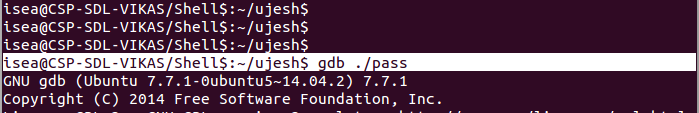
\includegraphics[width=120mm]{dbgcmd.png}
			
		\end{figure}
\\
Following command will extract the object code:\\
\begin{figure}[ht!]
	\centering
	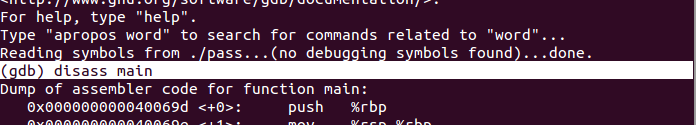
\includegraphics[width=120mm]{gdbass.png}
	
\end{figure}
   
\subsection {STEP 3: Searching Password}
Since the program verifies the correctness of a input password, that implies that it must have the correct password inside it's code.
That password must be a string and to match a string we need strcmp() function\\
So now our main target is to find the strcmp() function call in following assembly code.

\begin{figure}[ht!]
	\centering
	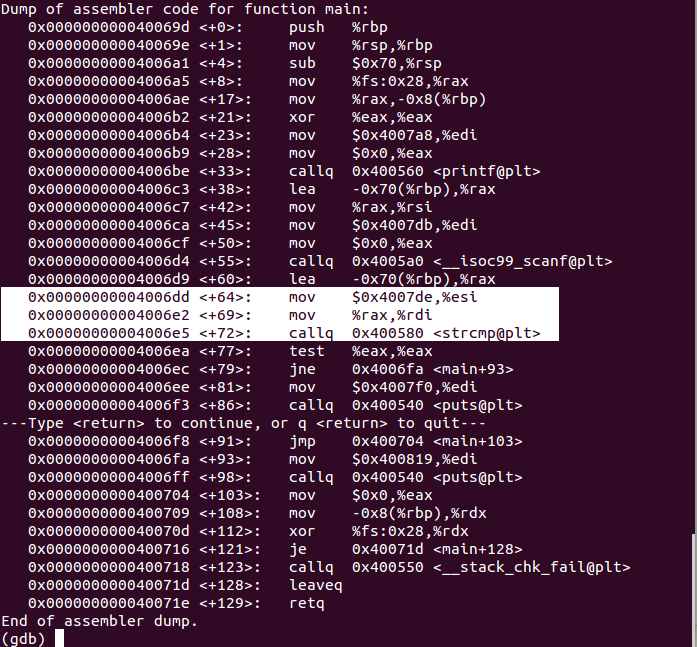
\includegraphics[width=120mm]{gdbcode.png}
	
\end{figure}
 \\  We can see that on address 0x0000000004006e5 there is call to strcmp() function. Hence both the strings must have passed to this function as an argument. Since the original password was declared static so it must have been moved from a memory address to a constant register.
 Thus we can conclude that on address 0x0000000004006dd the mov command actually moves the value of original password to register ESI.
 So to view the password we can run following command:
 
 \begin{figure}[ht!]
	\centering
	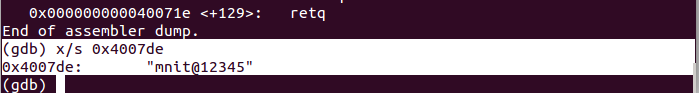
\includegraphics[width=120mm]{gdbcom.png}
	
\end{figure}
\\ As we can see in the screenshot that password was stored in the\\ address 0x4007de.
And we extracted the value of that address using x/s\\ \textless address\textgreater command.

So Password is "mnit@12345"
   

\end{document}
